\documentclass[a4paper]{ltjsarticle}
\usepackage[a4paper]{listings,jvlisting}
\usepackage{graphicx}

\lstset{
  basicstyle={\ttfamily},
  identifierstyle={\small},
  commentstyle={\smallitshape},
  keywordstyle={\small\bfseries},
  ndkeywordstyle={\small},
  stringstyle={\small\ttfamily},
  frame={tb},
  breaklines=true,
  columns=[l]{fullflexible},
  numbers=left,
  xrightmargin=0,
  xleftmargin=3,
  numberstyle={\scriptsize},
  stepnumber=1,
  numbersep=1,
  lineskip=-0.5ex
}

\renewcommand{\lstlistingname}{list}
\begin{document}

\title{プログラミング技法2\_課題5}
\author{阪田征之助}
\maketitle
\newpage
\section*{ソースコード}
ソースコードの主要部をlist\ref{code}に示す。

\begin{lstlisting}[caption=code,label=code]
    import pandas as pd
    import matplotlib.pylab as plt
    import numpy as np
    import scipy
    
    N = 100
    epsilon = 0.0001
    lr = 0.1
    
    if __name__=="__main__":
        
        #csvファイルからの読み込み
        df = pd.read_csv("weight-height.csv")
        
        # 05_01
        #100個をランダムに取得
        df_smp = df.sample(N)
        x = df_smp["Weight"].tolist()
        y = df_smp["Height"].tolist()
        plt.figure(1).clf()
        plt.scatter(x, y)
        plt.xlabel('Height')
        plt.ylabel('Weight')
        
        # 05_02
        #標準化
        x = (x - np.mean(x))/np.sqrt(np.var(x))
        y = (y - np.mean(y))/np.sqrt(np.var(y))
        print('Averaged standardized w:\t{:.2f}+-{:.2f}'.format(np.mean(x), np.std(x))) # np.mean(w) = 0, np.std(w) = 1
        print('Averaged standardized h:\t{:.2f}+-{:.2f}'.format(np.mean(y), np.std(y))) # np.mean(h) = 0, np.std(h) = 1
        
        # 05_03
        # MSE
        a = np.cov([x,y])[0][1]/np.var(x)
        b = np.mean(y) - a * np.mean(x) 
        mse = sum((y[i] - (b + a*x[i]))**2 for i in range(N))/N
        print('03:\tMSE: {:.2f}\ta: {:.2f}\tb: {:.2f}'.format(mse, a, b))
        
        # 05_04
        # 最急降下法
        a = 0
        b = 0
        mse = sum((y[i] - (a + b*x[i]))**2 for i in range(N))/N
        mse_list = [mse]
        while 1:
            new_a = a - lr * sum(x[i]*((b + a*x[i])- y[i]) for i in range(N))/N
            new_b = b - lr * sum((b + a*x[i])- y[i] for i in range(N))/N
            a = new_a
            b = new_b
            new_mse = sum((y[i] - (b + a*x[i]))**2 for i in range(N))/N
            mse_list.append(new_mse)
            if (new_mse - mse)**2 < epsilon**2:
                break
            else:
                mse = new_mse
        
        count = [i+1 for i in range(len(mse_list))]
        print('04:\tMSE: {:.2f}\ta: {:.2f}\tb: {:.2f}'.format(new_mse, a, b))
        plt.figure(2).clf()
        plt.scatter(count,mse_list, label='04')
        
        # 05_05
        # 行列で最急降下法
        #行列化
        X = []
        for _ in range(N):
            X.append([1,x[_]])
        X = np.matrix(X)
        Y = np.matrix([y]).T
        w = np.matrix([0,0]).T
    
        mse = sum((Y[i,0] - np.dot(X[i],w)[0,0])**2 for i in range(N))/N
        mse_list = [mse]
        while 1:
            w = w - lr * np.dot(X.T,(np.dot(X,w)-Y))/N
            new_mse = sum((Y[i,0] - np.dot(X[i],w)[0,0])**2 for i in range(N))/N
            mse_list.append(new_mse)
            if (new_mse - mse)**2 < epsilon**2:
                break
            else:
                mse = new_mse
        
        count = [i+1 for i in range(len(mse_list))]
        print('05:\tMSE: {:.2f}\ta: {:.2f}\tb: {:.2f}'.format(new_mse, w[1,0], w[0,0]))
        plt.figure(2)
        plt.scatter(count,mse_list, label='05')
        plt.xlabel('Iterations')
        plt.ylabel('MSE')
        plt.legend()
        
        # 05_06
        # 直接求める
        w = np.dot(np.linalg.inv(np.dot(X.T,X)),np.dot(X.T,Y))
        mse = sum((Y[i,0] - np.dot(X[i],w)[0,0])**2 for i in range(N))/N
        print('06:\tMSE: {:.2f}\ta: {:.2f}\tb: {:.2f}'.format(mse, w[1,0], w[0,0]))
        
        # 05_07
        # polyfitで求める
        a, b =np.polyfit(x, y, 1)
        mse = sum((y[i] - a*x[i] - b)**2 for i in range(N))/N
        print('07:\tMSE: {:.2f}\ta: {:.2f}\tb: {:.2f}'.format(mse, a, b))
        
        # 05_08
        df_male = df[df["Gender"] == "Male"]
        df_female = df[df["Gender"] == "Female"]
    
        x_male = df_male["Weight"].tolist()
        x_female = df_female["Weight"].tolist()
        y_male = df_male["Height"].tolist()
        y_female = df_female["Height"].tolist()
    
        x_m_ave = np.mean(x_male)
        x_m_var = np.sqrt(np.var(x_male))
        y_m_ave = np.mean(y_male)
        y_m_var = np.sqrt(np.var(y_male))
        x_f_ave = np.mean(x_female)
        x_f_var = np.sqrt(np.var(x_female))
        y_f_ave = np.mean(y_female)
        y_f_var = np.sqrt(np.var(y_female))
    
        pvalue_x = scipy.stats.ttest_ind(x_male, x_female)[1]
        pvalue_y = scipy.stats.ttest_ind(y_male, y_female)[1]
    
        plt.figure(3).clf()
        plt.subplot(121)
        plt.bar([0, 1], [x_m_ave,x_f_ave], yerr=[x_m_var, x_f_var])
        plt.ylabel('Height')
        plt.xticks([0, 1], ['Male', 'Female'])
        
        plt.subplot(122)
        plt.bar([0, 1], [y_m_ave,y_f_ave], yerr=[y_m_var, y_f_var])
        plt.ylabel('Weight')
        plt.xticks([0, 1], ['Male', 'Female'])
        plt.tight_layout()
        plt.show()
        
        if pvalue_x > .95:
            print('Female is higher than Male (p={:.3f})'.format(1 - pvalue_x))
        elif pvalue_x < .05:
            print('Male is higher than Female (p={:.3f})'.format(pvalue_x))
        else:
            print('There is no significant difference between Male and Female in height (p={:.3f})'.format(pvalue_x))
            
        if pvalue_y > .95:
            print('Female is heavier than Male (p={:.3f})'.format(1 - pvalue_y))
        elif pvalue_y < .05:
            print('Male is heavier than Female (p={:.3f})'.format(pvalue_y))
        else:
            print('There is no significant difference between Male and Female in weight (p={:.3f})'.format(pvalue_y))
\end{lstlisting}

平均と分散を求める関数をそれぞれ作成し、mein関数から呼び出す方式をとっている。
また、モジュールを使用して計算するパートではnumpyを使用している。

\section*{出力結果}
出力結果をlist\ref{result}に示す。
\begin{lstlisting}[caption=output, label=result]
    Averaged standardized w:        0.00+-1.00
    Averaged standardized h:        -0.00+-1.00
    03:     MSE: 0.13       a: 0.94 b: -0.00
    04:     MSE: 0.13       a: 0.92 b: -0.00
    05:     MSE: 0.13       a: 0.92 b: -0.00
    06:     MSE: 0.13       a: 0.93 b: -0.00
    07:     MSE: 0.13       a: 0.93 b: -0.00
    Male is higher than Female (p=0.000)
    Male is heavier than Female (p=0.000)
\end{lstlisting}
作成した関数の出力とモジュールを使用したパートの出力がほぼ一致しているため、正しく計算できていることがわかる。\\

\newpage
課題1で作成した散布図を図1に示す。
\begin{center}
    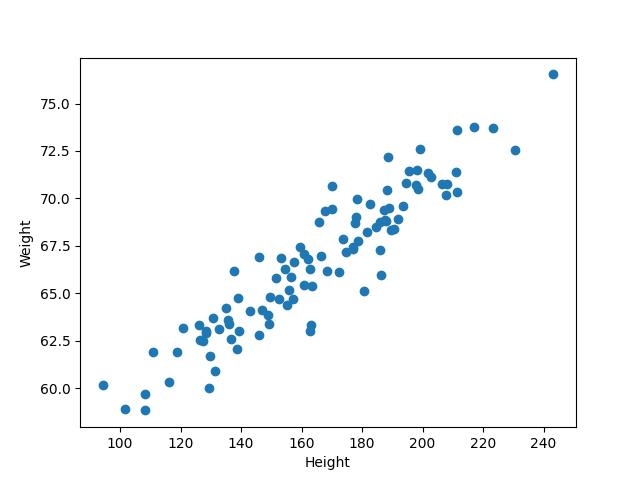
\includegraphics{Figure_1.jpeg} \\
    図1 Figure1
\end{center}
\newpage
課題4,5で作成した散布図を図2に示す。
\begin{center}
    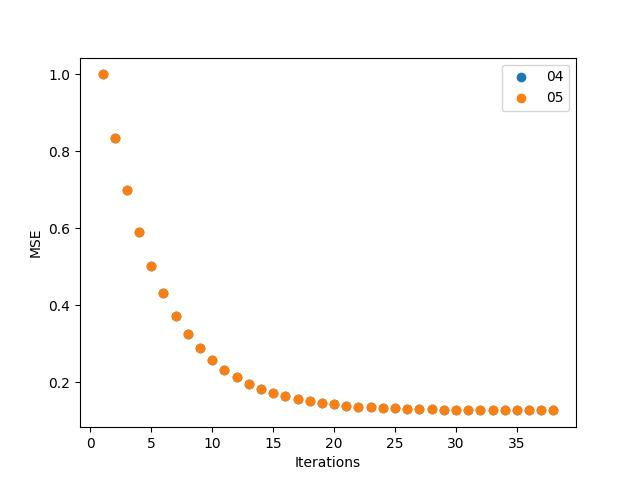
\includegraphics{Figure_2.jpeg} \\
    図2 Figure2
\end{center}
\newpage
課題8で作成した散布図を図3に示す。
\begin{center}
    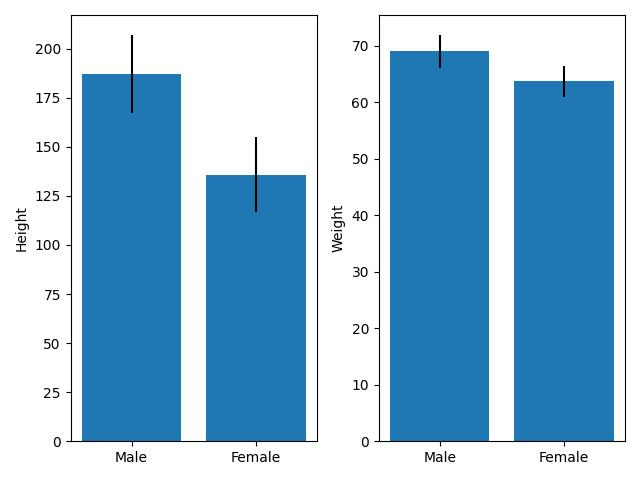
\includegraphics{Figure_3.jpeg} \\
    図3 Figure3
\end{center}

\section*{工夫した箇所}
今回課題ごとにプログラムを作成し、動作確認をしてから一つのプログラムに統合するという手段をとった。そのため、各プログラムでデバッグがしやすかった。
しかし、モジュール化を行っていないため、すごく長いプログラムとなってしまった。

\end{document}